\section{个人简介}

\subsection{教育背景}

\begin{xframe}{\kai{教育背景}}
    \cveducation
    {\entrylocationstyle{华中科技大学}}
    { }

    \vspace{2.0mm}

    \cvsubeducation
    {计算机科学与技术学院}
    {09/2016 - 02/2017}

    \vspace{-2.5mm}
    \begin{itemize}
        \item \descriptionstyle{计算机科学与技术,选修,GPA:3.6/4.0}
        \item \descriptionstyle{\itshape{核心课程: 高等工程数学(矩阵论 \& 数理统计 \& 数值计算), 人工智能, 模式识别, 知识发现与数据开采, 大数据技术, 启发式优化}}
    \end{itemize}

    \cvsubeducation
    {管理学院}
    {09/2015 - 06/2016}

    \vspace{-2.5mm}
    \begin{itemize}
        \item \descriptionstyle{会计硕士,主修, GPA 3.8/4.0}
        \item \descriptionstyle{\itshape{核心课程: 财务管理理论与实务, 管理会计理论与实务, 审计理论与实务,内部控制理论与实务,金融市场与金融工具}}
    \end{itemize}

\end{xframe}

\begin{xframe}{\kai{教育背景}}
    \cveducation
    {\entrylocationstyle{中南财经政法大学}}
    { }

    \vspace{2.0mm}

    \cvsubeducation
    {会计学院}
    {09/2011 - 06/2015}

    \vspace{-2.5mm}

    \begin{itemize}
        \item \descriptionstyle{会计学学士}
        \item \descriptionstyle{\itshape{核心课程: 会计学原理,中级会计学,管理会计学(双语),企业资源计划,会计实验学,会计电算化}}
    \end{itemize}

\end{xframe}

\subsection{研究经历}

\begin{xframe}{\kai{研究经历}}
    \cvexperience
    {\entrylocationstyle{研究助理},蔡淑琴教授,管理学院}
    {09/2015 - 08/2017}

    \vspace{-2.5mm}

    \begin{itemize}
        \item \descriptionstyle{结合句法结构与向量空间模型,提出一种考虑抱怨问题路径的网络抱怨识别方法;}
        \item \descriptionstyle{考虑知识、情感和互动三个资源维度,建立处理在线负面口碑的专家识别方法;}
        \item \descriptionstyle{参与大数据实验室的建设,撰写17年国家自科基金项目申请书中关于大数据产品质量测度的部分;}
    \end{itemize}

    \cvexperience
    {\entrylocationstyle{研究助理},大数据实验室,管理学院}
    {03/2016 - 08/2017}

    \vspace{-2.5mm}

    \begin{itemize}
        \item \descriptionstyle{利用有源标签信号强度在多个接收器的差别,实现基于ZigBee的区域定位接口;}
        \item \descriptionstyle{搭建基于Hadoop的全分布式计算机集群,实现Map/Reduce框架下的Naïve Bayes分类器;}
    \end{itemize}

\end{xframe}

\begin{xframe}{\kai{研究经历}}
    \cvexperience
    {\entrylocationstyle{研究实习},何琨教授,计算机学院}
    {07/2017 - PRESENT}

    \vspace{-2.5mm}

    \begin{itemize}
        \item \descriptionstyle{提出会计事项的机器理解方法,利用Word2Vec方法实现会计事项的词向量空间嵌入;}
        \item \descriptionstyle{提出会计分录的机器编制方法,利用GRUs+Attention机制实现会计知识的深度学习;}
        \item \descriptionstyle{探索神经网络的随机逼近方法,利用随机权重机制进行神经网络参数的快速寻优;}
        \item \descriptionstyle{探索深度神经网络的解释性,尝试利用随机权重机制解释神经网络的训练过程;}
    \end{itemize}
\end{xframe}

\subsection{教学经历}

\begin{xframe}{\kai{教学经历}}
    \cvexperience
    {\entrylocationstyle{助理教师},蔡淑琴教授,管理学院}
    {03/2016 - 09/2017}

    \vspace{-2.5mm}

    \begin{itemize}
        \item \descriptionstyle{MBA课程:电子商务}
        \item \descriptionstyle{本科生课程:管理信息系统分析与设计,专业概论,课程设计,生产实习(信息管理与信息系统)}
    \end{itemize}

    \vspace{1.0mm}
    \cvexperience
    {\entrylocationstyle{助理教师},石双元教授,管理学院}
    {09/2016 - 01/2017}

    \vspace{-2.5mm}

    \begin{itemize}
        \item \descriptionstyle{本科生课程:信息系统开发方法与工具(C\#)}
    \end{itemize}

    \vspace{1.0mm}
    \cvexperience
    {\entrylocationstyle{助理教师},张千帆教授,管理学院}
    {09/2015 - 01/2016}

    \vspace{-2.5mm}

    \begin{itemize}
        \item \descriptionstyle{本科生课程:数据结构(C/C++),数据库技术及应用}
    \end{itemize}
\end{xframe}

\subsection{工程经历}

\begin{xframe}{\kai{工程经历}}
    \cvexperience
    {\entrylocationstyle{系统工程师},华威科智能股份有限公司}
    {11/2016 - 08/2017}

    \vspace{-2.5mm}

    \begin{itemize}
        \item \descriptionstyle{主导设计并参与开发一套武术体育竞赛管理信息系统;}
        \item \descriptionstyle{负责整套系统的需求分析、信息模型设计、功能设计、数据库设计和功能测试等;}
        \item \descriptionstyle{独立负责运动员管理与检录的开发工作,基于RFID实现运动员自动化注册和检录;}
        \item \descriptionstyle{承担2016年湖南省武术比赛、2017年湖北省青少年武术锦标赛的竞赛管理;}
    \end{itemize}

    \cvexperience
    {\entrylocationstyle{程序员},管理学院MPACC中心}
    {03/2018}

    \vspace{-2.5mm}

    \begin{itemize}
        \item \descriptionstyle{设计并基于RFID开发一套研究生复试检录抽签系统;}
    \end{itemize}

\end{xframe}

\subsection{获奖 \& 荣誉}

\begin{xframe}{\kai{获奖 \& 荣誉}}
    \begin{cvhonors}
        %------------------------------------------------

        \cvhonor
        {国家奖学金} % Award
        {华中科技大学} % Event
        {湖北,武汉} % Location
        {2017} % Date(s)
        %------------------------------------------------

        \cvhonor
        {知行奖学金} % Award
        {华中科技大学} % Event
        {湖北,武汉} % Location
        {} % Date(s)

        %------------------------------------------------

        \cvhonor
        {三好研究生} % Award
        {华中科技大学} % Event
        {湖北,武汉} % Location
        {2016} % Date(s)

        %------------------------------------------------

        % \cvhonor
        % {学业奖学金} % Award
        % {华中科技大学} % Event
        % {湖北,武汉} % Location
        % { } % Date(s)

        %------------------------------------------------

        \cvhonor
        {优秀运动员} % Award
        {全国大学生武术锦标赛} % Event
        {兰州,甘肃} % Location
        { } % Date(s)

        %------------------------------------------------

        \cvhonor
        {第四名} % Award
        {南棍,全国大学生武术锦标赛} % Event
        {兰州,甘肃} % Location
        { } % Date(s)

        %------------------------------------------------

        \cvhonor
        {第六名} % Award
        {南拳, 全国大学生武术锦标赛} % Event
        {兰州,甘肃} % Location
        { } % Date(s)

        %------------------------------------------------

        \cvhonor
        {第一名} % Award
        {南拳,湖北省大学生武术比赛} % Event
        {湖北,武汉} % Location
        { } % Date(s)

        %------------------------------------------------

        \cvhonor
        {优秀学士学位论文} % Award
        {中南财经政法大学} % Event
        {湖北,武汉} % Location
        {2015} % Date(s)


        %------------------------------------------------

        \cvhonor
        {第三名} % Award
        {南拳,湖北省大学生武术比赛} % Event
        {湖北,武汉} % Location
        { } % Date(s)
    \end{cvhonors}
\end{xframe}

\subsection{论文 \& 技能}

\begin{xframe}{\kai{论文 \& 技能}}
    \begin{cventries}

            \begin{itemize}
                \item \descriptionstyle{张心泽,蔡淑琴,罗思宇. 基于支持向量机的在线负面口碑处理专家识别\upshape{[J]}. 统计与决策. 2017.}
                \item \descriptionstyle{崔晓兰,蔡淑琴,张心泽. 一种考虑抱怨问题路径的网络抱怨问题识别方法. 运筹与管理. 在审.}
                \item \descriptionstyle{张心泽. 账务智能处理中会计机器代理的研究\upshape{[D]}. 华中科技大学. 2017.}
                \item \descriptionstyle{Xinze Zhang. Debit and credit, end-to-end learning for accounting processing. Working}
            \end{itemize}

    \end{cventries}

    \begin{cvskills}

        %------------------------------------------------
        \cvskill
        {Programming} % Category
        {Python, C\#, SQL, Java, \LaTeX, Hadoop, RFID, Linux} % Skills

        %------------------------------------------------
        \cvskill
        {Wikipedia} % Category
        {{zh.wikipedia.org/wiki/Special:用户贡献/Xinze.zh}} % Skills

        %------------------------------------------------
        \cvskill
        {GitHub} % Category
        {github.com/XinzeZhang} % Skills

    \end{cvskills}

\end{xframe}

{
\usebackgroundtemplate{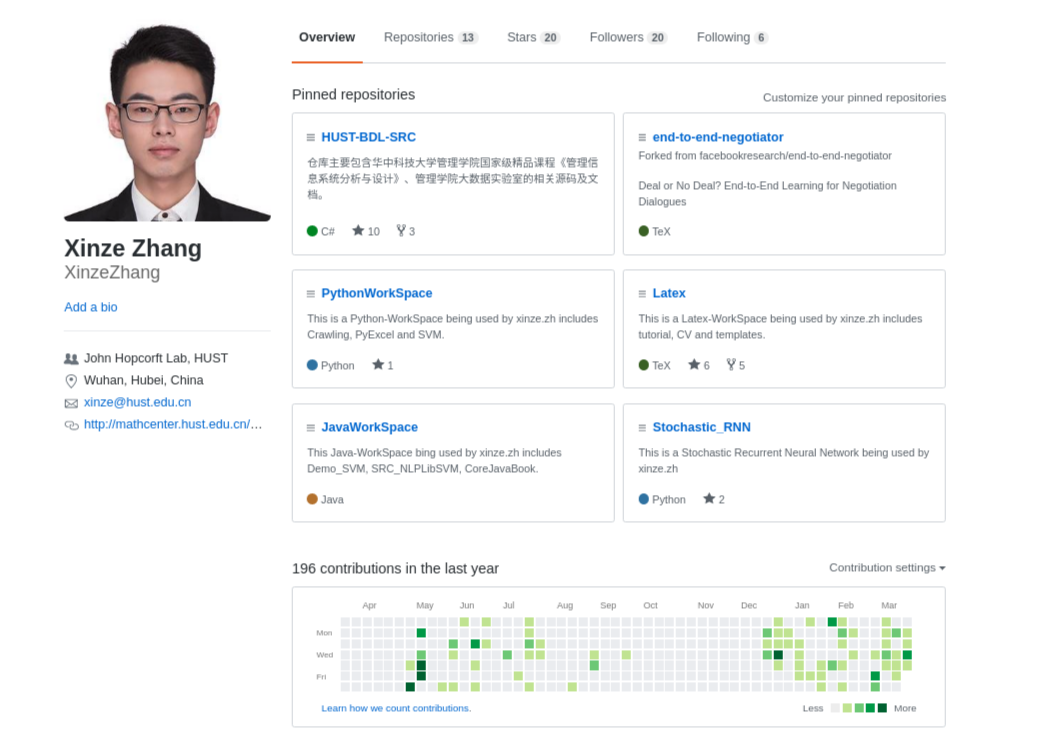
\includegraphics[width=\paperwidth]{./style/images/github.png}}
\begin{frame}[plain]
    
\end{frame}
}